\documentclass[format=acmsmall, review=false, screen=true]{acmart}


\usepackage{booktabs} % For formal tables
\usepackage[utf8]{inputenc}
\usepackage[T1]{fontenc}
\usepackage[spanish]{babel}
\usepackage{pdfpages}

\usepackage[ruled]{algorithm2e} % For algorithms
\renewcommand{\algorithmcfname}{ALGORITHM}
\SetAlFnt{\small}
\SetAlCapFnt{\small}
\SetAlCapNameFnt{\small}
\SetAlCapHSkip{0pt}
\IncMargin{-\parindent}


% Metadata Information
\acmJournal{TEMA}
%\acmVolume{9}
%\acmNumber{4}
\acmArticle{\textbf{Propuesta 2}}
\acmYear{2018}
\acmMonth{2}
\copyrightyear{2018}
%\acmArticleSeq{9}

% Copyright
\setcopyright{none}
%\setcopyright{acmlicensed}
%\setcopyright{rightsretained}
%\setcopyright{usgov}
%\setcopyright{usgovmixed}
%\setcopyright{cagov}
%\setcopyright{cagovmixed}

\settopmatter{printacmref=false}
\renewcommand\footnotetextcopyrightpermission[1]{} % removes footnote with conference information in first column
%\pagestyle{plain} % removes running headers


% DOI
%\acmDOI{0000001.0000001}

% Paper history
%\received{February 2007}
%\received[revised]{March 2009}
%\received[accepted]{June 2009}


% Document starts
\begin{document}
% Title portion. Note the short title for running heads
\title[A Multifrequency MAC for Wireless Sensor]{Modelado y Simulación de Colas de Mensajes Distribuidas
  \\ \small{Instituto Tecnológico de Costa Rica\\ Escuela de Ingeniería en Computación\\ Maestría en Computación\\ MC-7205 Tema Selecto de Investigación\\}
}

\author{Carlos Martín Flores González}
\affiliation{%
  \institution{Carné: 2015183528}
%  \city{Cartago}
%  \state{Cartago}
%  \postcode{506}
%  \country{2015183528}
}
\email{mfloresg@gmail.com}

\authorsaddresses{}

%\begin{abstract}
%Multifrequency media access control has been well understood in
%general wireless ad hoc networks, while in wireless sensor networks,
%researchers still focus on single frequency solutions. In wireless
%sensor networks, each device is typically equipped with a single
%radio transceiver and applications adopt much smaller packet sizes
%compared to those in general wireless ad hoc networks. Hence, the
%multifrequency MAC protocols proposed for general wireless ad hoc
%networks are not suitable for wireless sensor network applications,
%which we further demonstrate through our simulation experiments. In
%this article, we propose MMSN, which takes advantage of
%multifrequency availability while, at the same time, takes into
%consideration the restrictions of wireless sensor networks. Through
%extensive experiments, MMSN exhibits the prominent ability to utilize
%parallel transmissions among neighboring nodes.
%\end{abstract}


%
% The code below should be generated by the tool at
% http://dl.acm.org/ccs.cfm
% Please copy and paste the code instead of the example below.
%
%\begin{CCSXML}
%<ccs2012>
% <concept>
%  <concept_id>10010520.10010553.10010562</concept_id>
%  <concept_desc>Computer systems organization~Embedded systems</concept_desc>
%  <concept_significance>500</concept_significance>
% </concept>
% <concept>
%  <concept_id>10010520.10010575.10010755</concept_id>
%  <concept_desc>Computer systems organization~Redundancy</concept_desc>
%  <concept_significance>300</concept_significance>
% </concept>
% <concept>
%  <concept_id>10010520.10010553.10010554</concept_id>
%  <concept_desc>Computer systems organization~Robotics</concept_desc>
%  <concept_significance>100</concept_significance>
% </concept>
% <concept>
%  <concept_id>10003033.10003083.10003095</concept_id>
%  <concept_desc>Networks~Network reliability</concept_desc>
%  <concept_significance>100</concept_significance>
% </concept>
%</ccs2012>
%\end{CCSXML}
%
%\ccsdesc[500]{Computer systems organization~Embedded systems}
%\ccsdesc[300]{Computer systems organization~Redundancy}
%\ccsdesc{Computer systems organization~Robotics}
%\ccsdesc[100]{Networks~Network reliability}

%
% End generated code
%

%
%\keywords{Wireless sensor networks, media access control,
%multi-channel, radio interference, time synchronization}




\maketitle

% The default list of authors is too long for headers.
%\renewcommand{\shortauthors}{G. Zhou et al.}

\hspace{-0.6cm}
\fbox{
  \parbox{\textwidth}{
    \textbf{Idea tomada de: (Ver documento al final)}\\
    \url{https://sdqweb.ipd.kit.edu/wiki/Modeling_and_Simulation_of_Distributed_Message_Queues}
  }
}

\section{Problema}
No se tiene cuantificado el impacto en el rendimiento del uso de sistemas distribuidos de intercambio de mensajes en un sistema de software. 

\section{Justificación}
En general, la influencia del impacto de la agregación y/o modificación de componentes en un sistema de software es usualmente una tarea que no se realiza. Muchas veces se asume que el delegar funciones a un producto o librería de código va a brindar resultados positivos de manera casi inmediata. No se toma en cuenta que cada nuevo componente que se agrega al sistema también aporta complejidad y comporatmiento los cuales podrían comprometer un sistema.\\ 

Los sistemas distribuidos de intercambio de mensajes se han convertido en una alternativa para alivianar la carga y reducir la complejidad de un sistema de software. Por medio de estas, los sistemas se encargan de publicar mensajes a una cola mientras que por otro lado otros sistemas se encargan de leer los mensajes publicados a esa cola periódicamente.\\

Una investigación sobre la influencia del impacto en el rendimiento del uso de  sistemas distribuidos de mensajes en un sistema de software puede ayudar a dar a conocer factores favoren o desfavorecen el uso de los mismos y, además de esto, podría representar un marco de referencia inicial por medio del cual se pueda evaluar la adopción de estas tecnologías \emph{a priori}. 

\section{Objetivo General}
Evaluar la influencia en el rendimiento de sistemas distribuidos de intercambio de mensajes por medio de modelado y simulación

\label{sec:original}
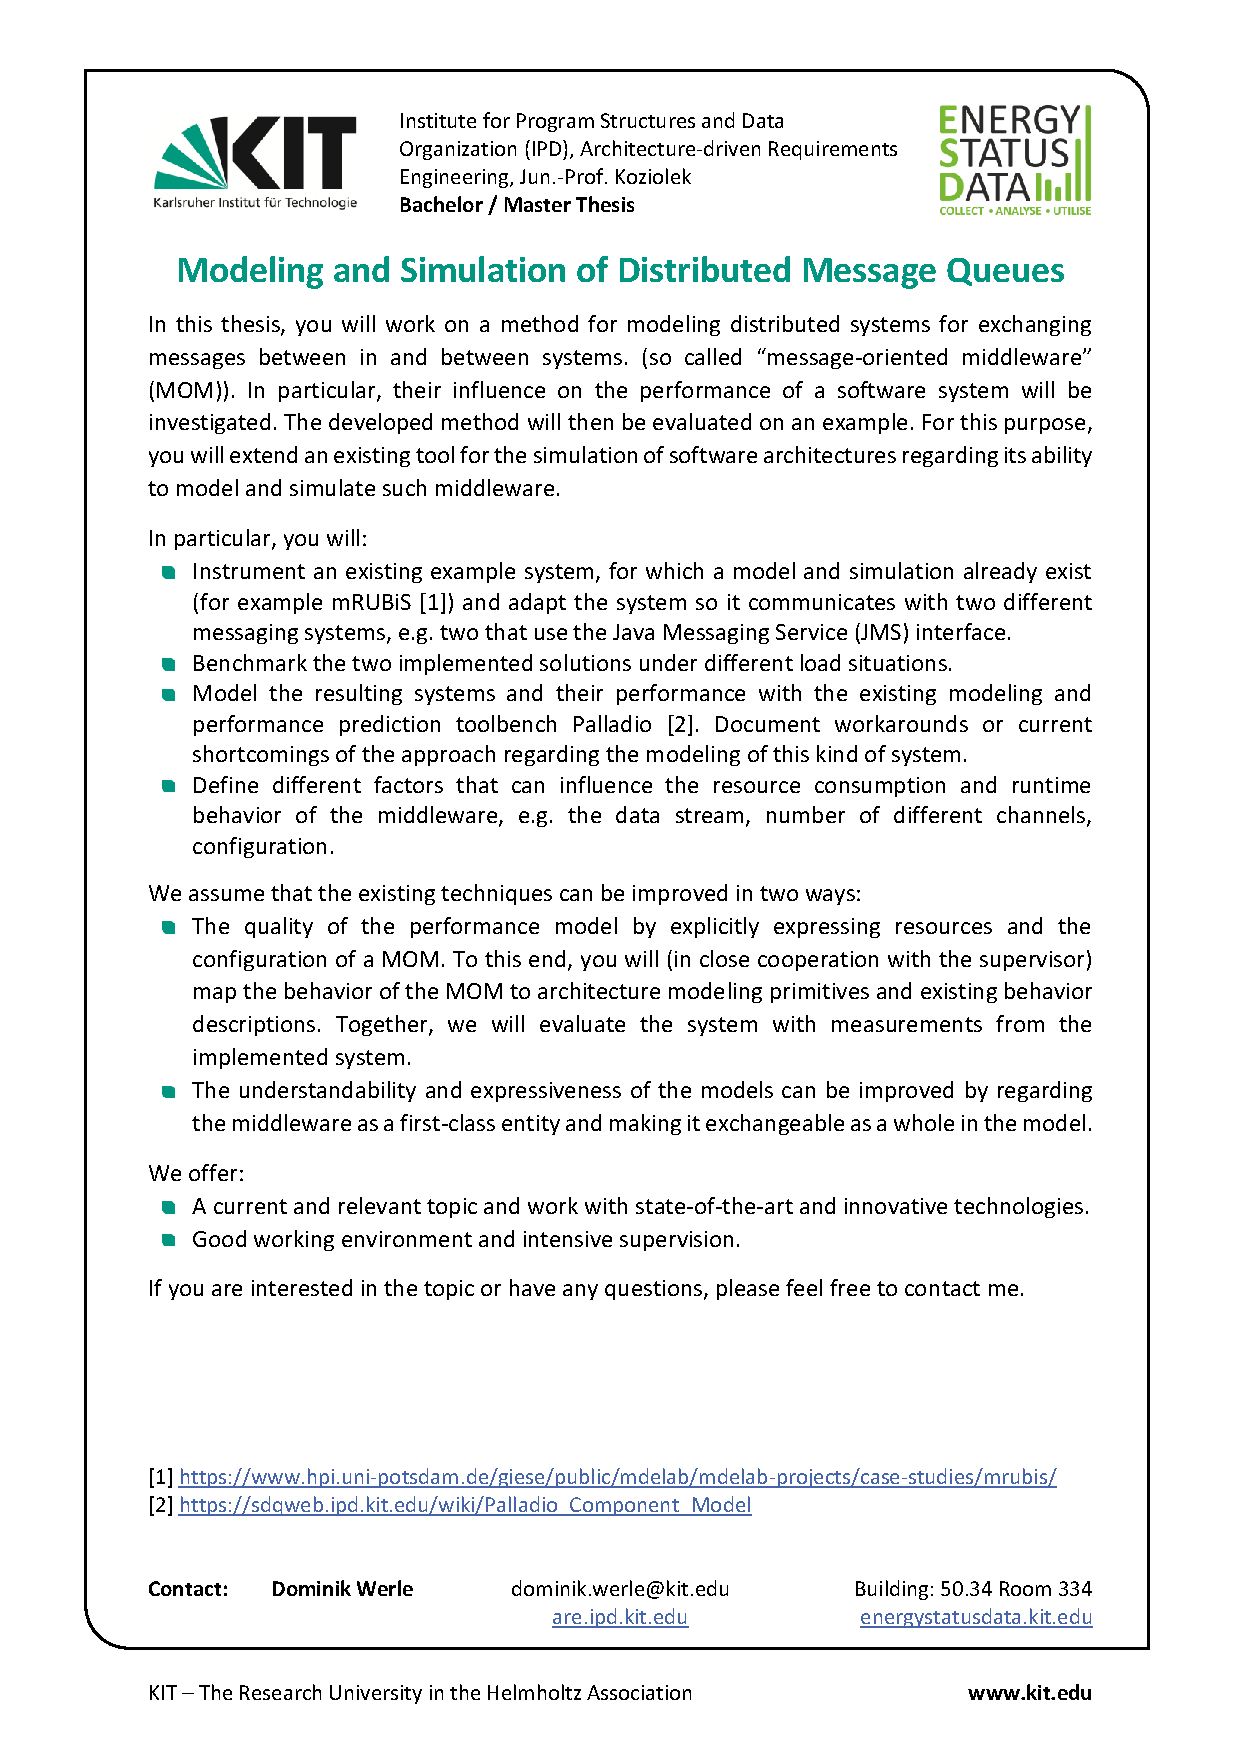
\includepdf[pages=1]{modeling-simulating-distributed-queues}


\end{document}
